\documentclass{article}

\usepackage{neurips_2023}



\usepackage[utf8]{inputenc} % allow utf-8 input
\usepackage[T1]{fontenc}    % use 8-bit T1 fonts
\usepackage{hyperref}       % hyperlinks
\usepackage{url}            % simple URL typesetting
\usepackage{booktabs}       % professional-quality tables
\usepackage{amsfonts}       % blackboard math symbols
\usepackage{nicefrac}       % compact symbols for 1/2, etc.
\usepackage{microtype}      % microtypography
\usepackage{xcolor}         % colors
\usepackage{graphicx}
\graphicspath{ {./imagenes/} }

\title{Pre TP1: Data Mining en Ciencia y Tecnología}

\author{%
  José Saint Germain\\
  \texttt{josesg998@gmail.com} \\
}

\begin{document}

\maketitle

\section{Introducción}

El procesamiento de imágenes resulta desafiante por su alta 
dimensionalidad. La estructura de una {\bf imagen digital} consiste 
en una  {\bf matriz de NxM}, en donde la subunidad constituyente de 
la matriz es un  {\bf pixel} que codifica información para un color 
particular. Cada pixel representa la intesidad de luz en ese 
punto, que generalmente varía entre  {\bf [0,255]}, 
lo que es equivalente a  {\bf8 bits.}\

Para representar imágenes a colores, se utiliza un modelo de 
percepción humana, en donde el color resulta a través de un
sistema aditivo. El modelo se basa en la teoría de los componentes
primarios del color que son Rojo, Verde y Azul  {\bf (RGB Red, Green 
and Blue}, por sus siglas en inglés). Por consiguiente, para 
representar digitalmente una imagen color, se necesitan  {\bf 3 
matrices de NxM}. Una para el Rojo, otra para el Verde y 
otra para el Azul.

\section{Objetivos}


Familiarizarse con el procesamiento de imágenes. Para ello, se proponen 
diferentes manipulaciones que permitirán preparar el dataset para la 
detección y exploración de agrupamientos naturales.

\section{Estructura de los datos}

A partir del siguiente \href{https://www.kaggle.com/datasets/olgabelitskaya/flower-color-images}{link},
se obtendrán las imágenes a color de {\bf 210 flores} pertenecientes a {\bf 10 especies 
diferentes}. Cada imagen consiste en un archivo {\bf .PNG} de 128 pixeles de ancho 
por 128 pixeles de profundidad ({\bf 128x128x3}). Adicionalamente, se encuentra el 
archivo {\bf .CSV} con las etiquetas (labels) que corresponden a la especie de cada imagen.

\section{Procesamiento de imágenes}

{\emph Cargar el dataset de imágenes y sus respectivas etiquetas. Es importante asegurarse que las 
imágenes sean comparables en color, valor, rango y tamaño.

Explorar y graficar los subconjuntos de imágenes que representan flores de la misma
especie.}
\pagebreak

\begin{figure}[h!]
  \centering  
  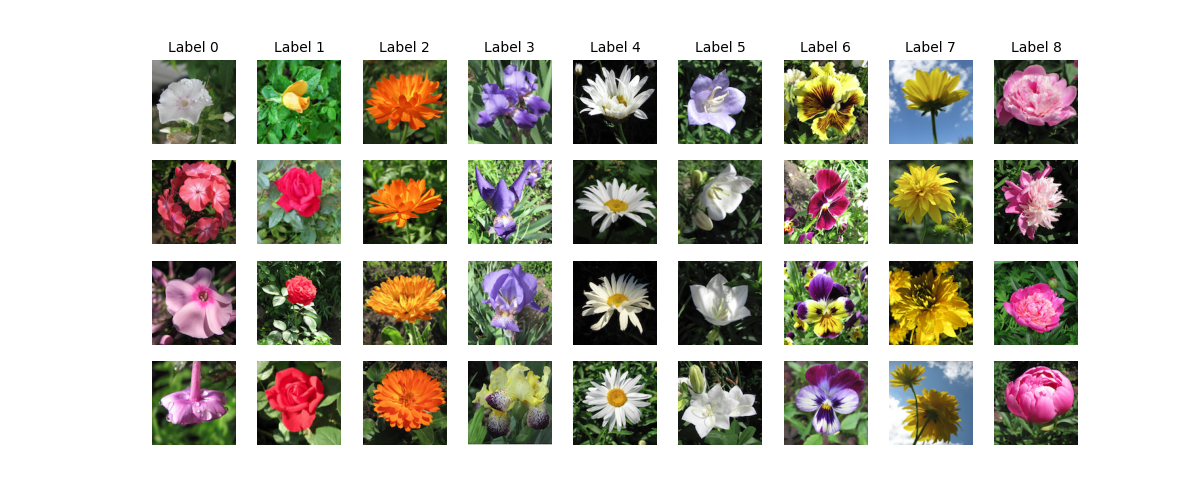
\includegraphics[width=1\textwidth]{1_ejemplos_flores.png}
  \caption{Exploración de especies de flores}
\end{figure}

\section{Manipulación de datos}

\subsection{Cambio de brillo}

{\emph Cambiar la intensidad de una de las imágenes en escala de grises, transformarla en una imagen con mucho y otra con poco brillo.}

\begin{figure}[h!]
  \centering    
  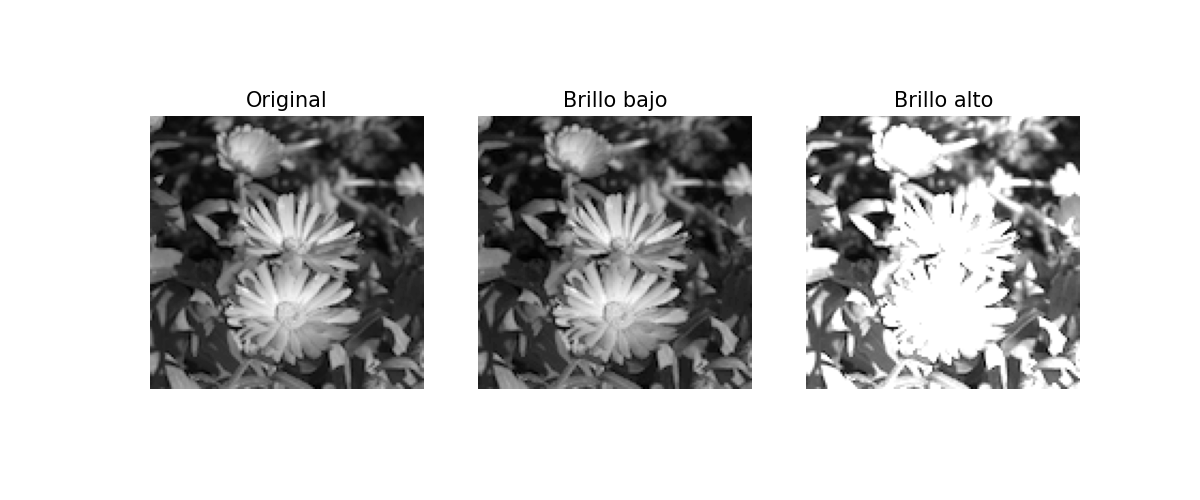
\includegraphics[width=1\textwidth]{2_brillo.png}
  \caption{Ajuste de brillo}
\end{figure}

\subsection{Imagen en blanco y negro}

{\emph Convertir una de las imágenes a blanco y negro (binario). ¿Es la única manera? Si existen otras transformaciones mostrar más de una conversión}
\pagebreak
\begin{figure}[h!]
  \centering    
  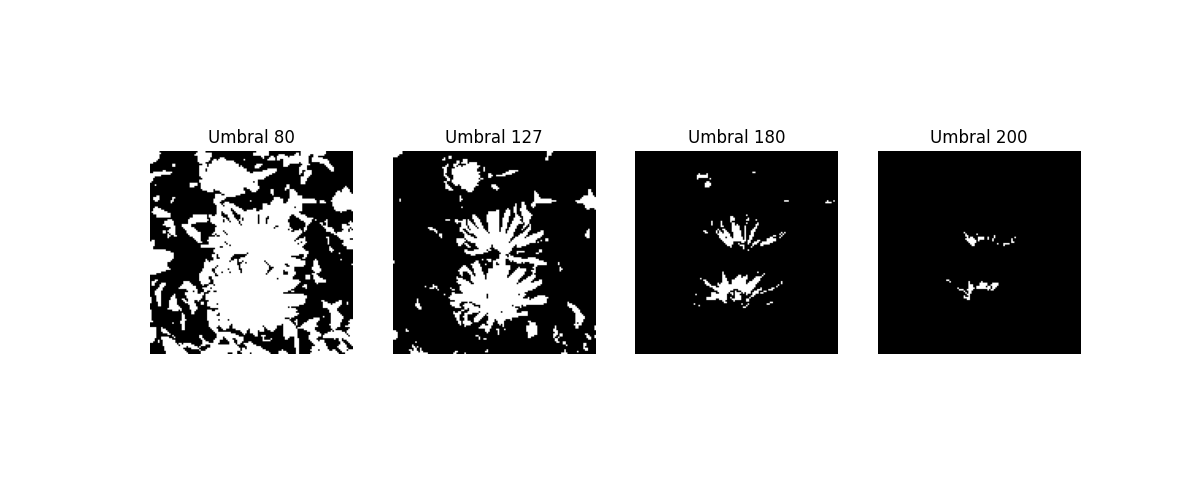
\includegraphics[width=.3\textwidth]{3_binario.png}
  \caption{Imagen binaria}
\end{figure}

\subsection{Imagen recortada}
\label{others}

{\emph Recortar una parte significativa de la imagen, quedándose sólo con el círculo central de la misma.}

\begin{figure}[h!]
  \centering    
  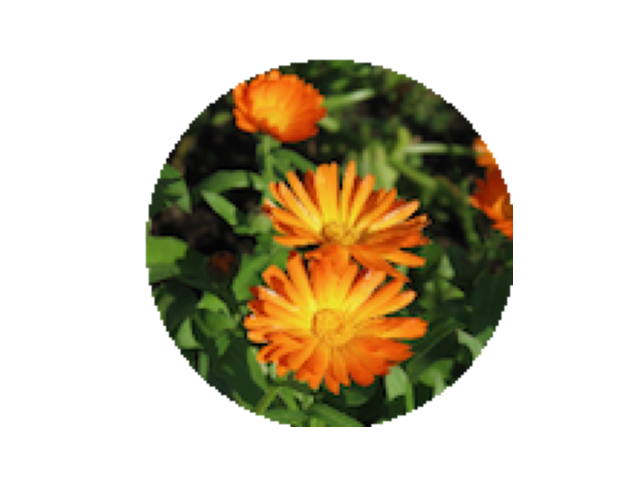
\includegraphics[width=.3\textwidth]{4_recortado.png}
  \caption{Recorte de imagen}
\end{figure}
\subsection{Imágenes mezcladas}

{\emph Generar dos imágenes random: una imagen mezclando los pixels y otra mezclando
partes de diferentes imágenes.}

\begin{figure}[h!]
  \centering    
  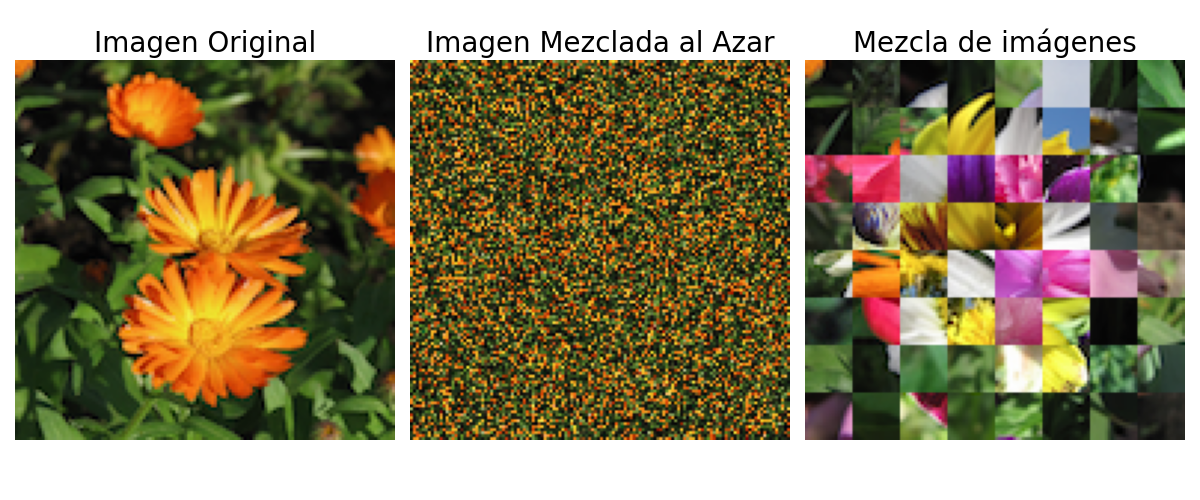
\includegraphics[width=.75\textwidth]{5_mezcla.png}
  \caption{Imagenes con píxeles mezclados e intercambiados}
\end{figure}

\subsection{Filtros de imagen}

{\emph Aplicar dos tipos diferentes de filtros sobre una imagen, 
explique en qué casos conviene usar cada uno.}
\pagebreak

\begin{figure}[h!]
  \centering    
  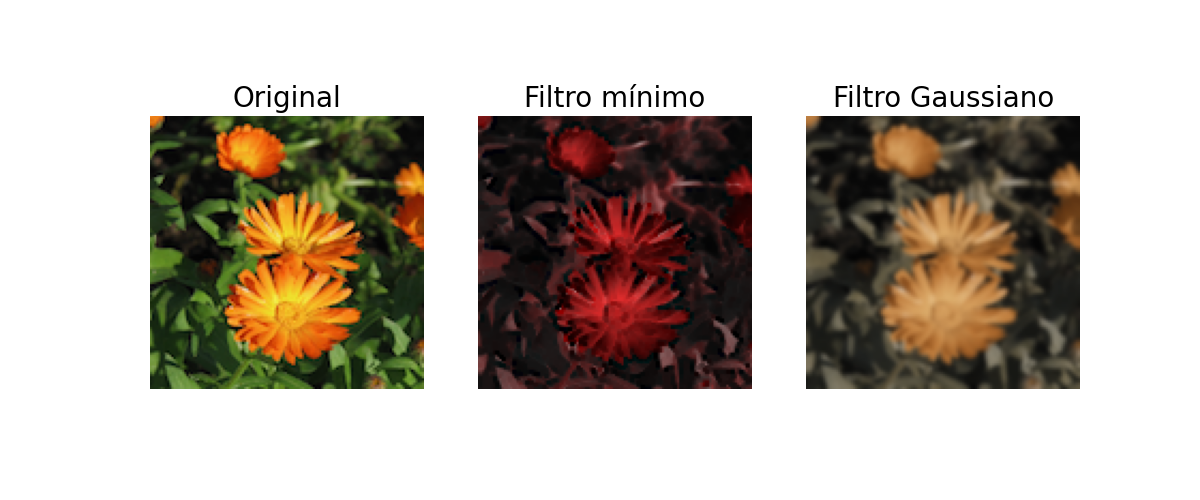
\includegraphics[width=1\textwidth]{6_filtro.png}
  \caption{Imagenes con filtros}
\end{figure}

\subsection{Imágenes promedio}

{\emph Calcular imagen promedio global y el promedio entre las distintas especies. ¿Se pueden
distinguir los promedios? ¿Cómo quedan los promedios si consideran las imágenes en
blanco y negro?}

\begin{figure}[h!]
  \centering    
  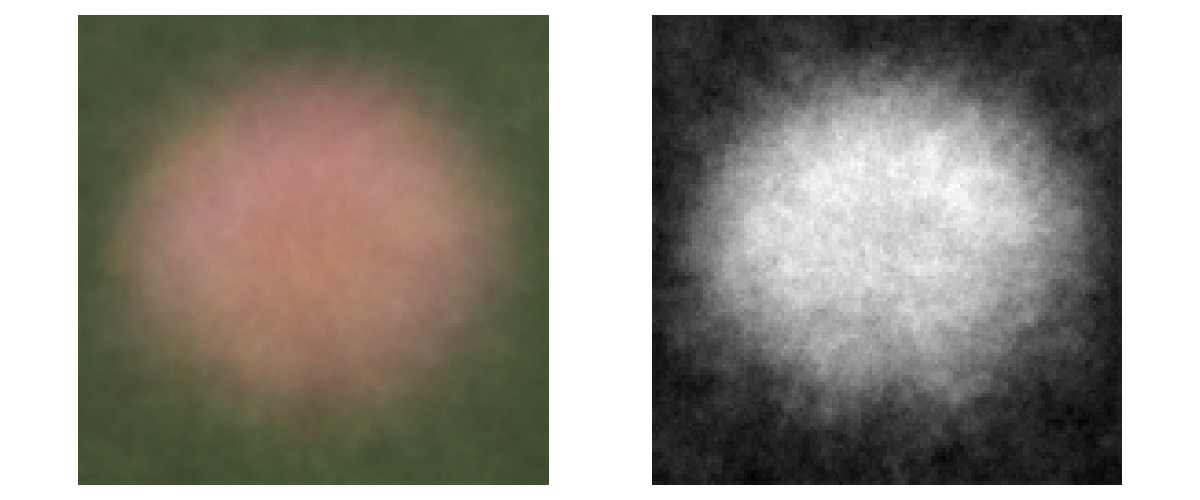
\includegraphics[width=.7\textwidth]{7_1_promedio.png}
  \caption{Imagenes promedio color y blanco y negro}
\end{figure}


\begin{figure}[h!]
  \centering    
  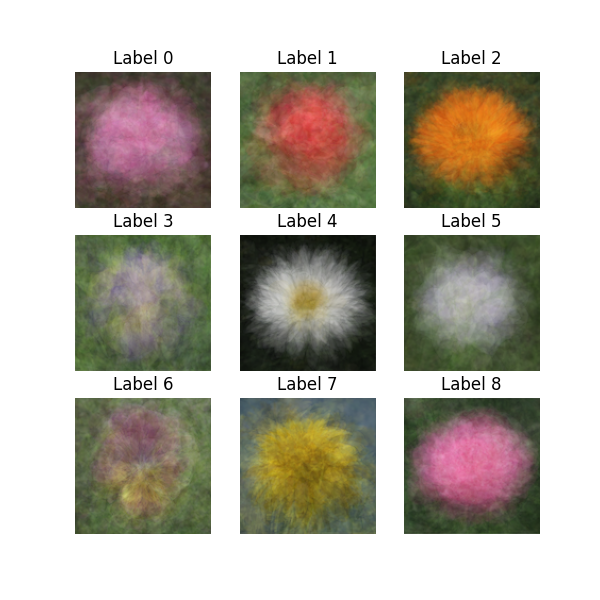
\includegraphics[width=.6\textwidth]{7_2_promedio_especies_color.png}
  \caption{Imagenes promedio color y blanco y negro}
\end{figure}

\begin{figure}[h!]
  \centering    
  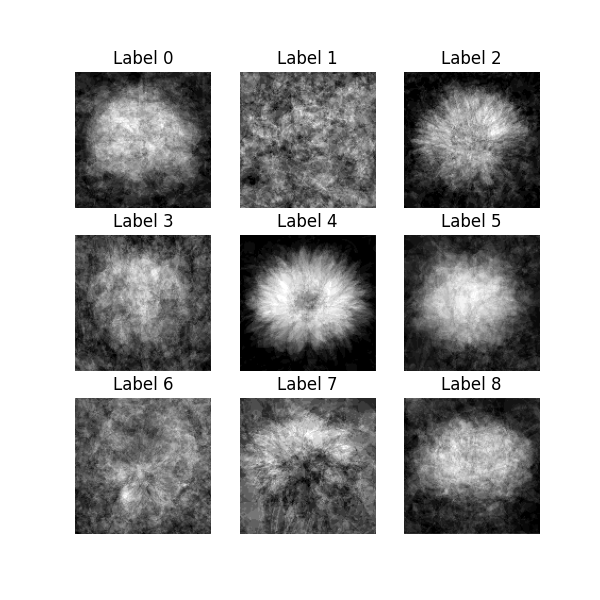
\includegraphics[width=.6\textwidth]{7_3_promedio_especies_bn.png}
  \caption{Imagenes promedio color y blanco y negro}
\end{figure}
\pagebreak
\section{Búsqueda de features}

{\emph Analizar las distribuciones de valores de pixels por cada especie. ¿Se puede distinguir
una especie en algún rango de color?}

\begin{figure}[h!]
  \centering    
  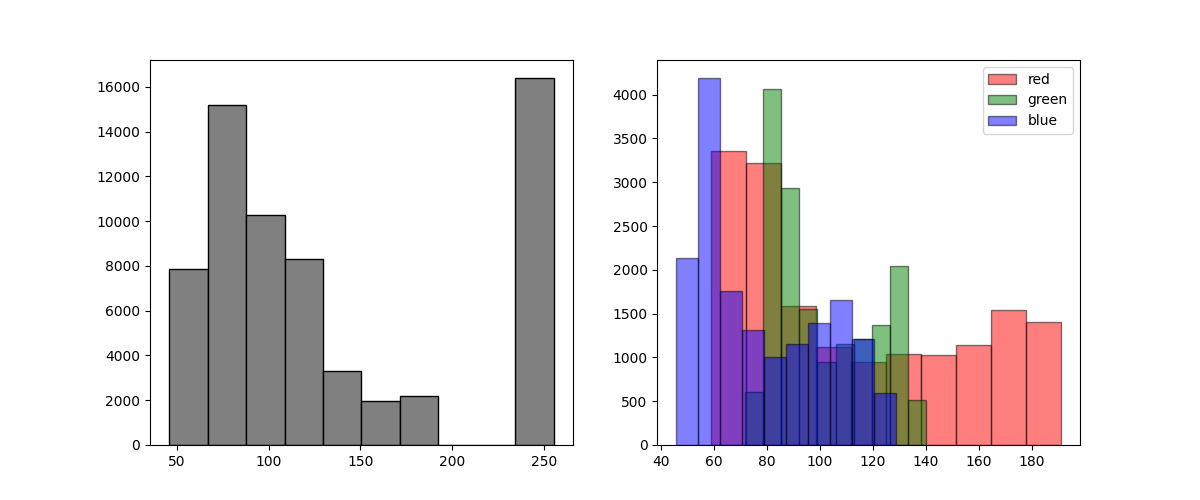
\includegraphics[width=1\textwidth]{8_1_pixeles_general.png}
  \caption{Distribución promedio de píxeles}
\end{figure}

% \begin{figure}[h!]
%   \centering    
%   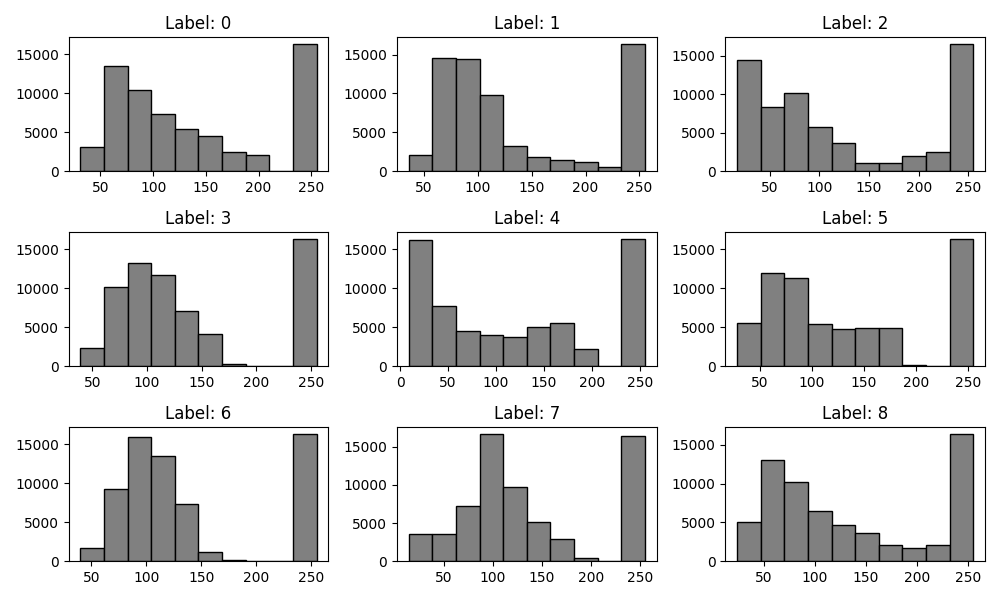
\includegraphics[width=1\textwidth]{8_2_pixeles_especies_byn.png}
%   \caption{Distribución de pixeles por especie}
% \end{figure}

\begin{figure}[h!]
  \centering    
  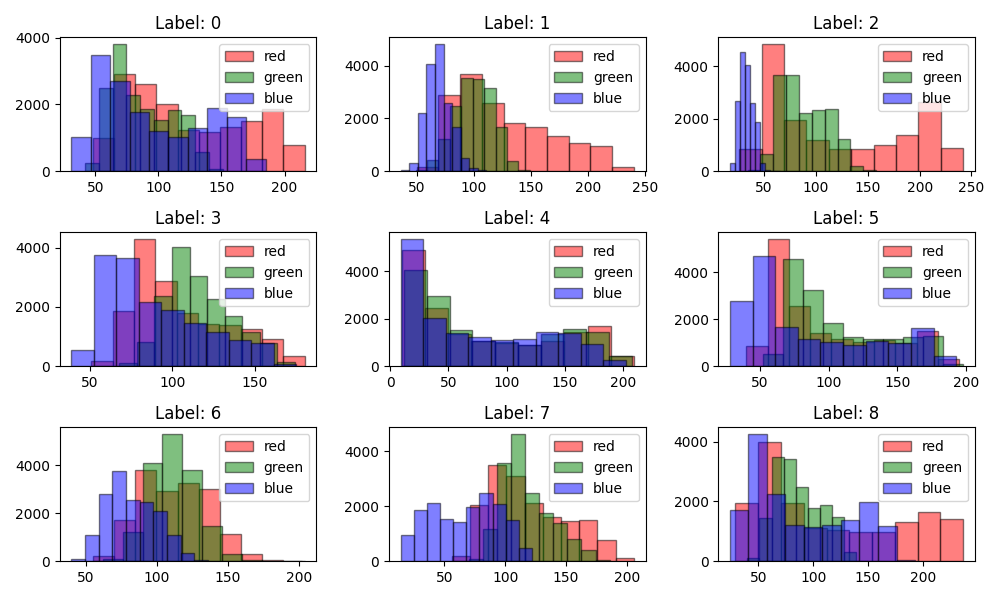
\includegraphics[width=1\textwidth]{8_3_pixeles_especies_color.png}
  \caption{Distribución de pixeles de color por especie}
\end{figure}
\pagebreak

\subsection{Análisis de componentes principales}

{\emph Realizar una inspección de las componentes principales del dataset y analizar si se
pueden identificar las especies en esta representación.}

\begin{figure}[h!]
  \centering    
  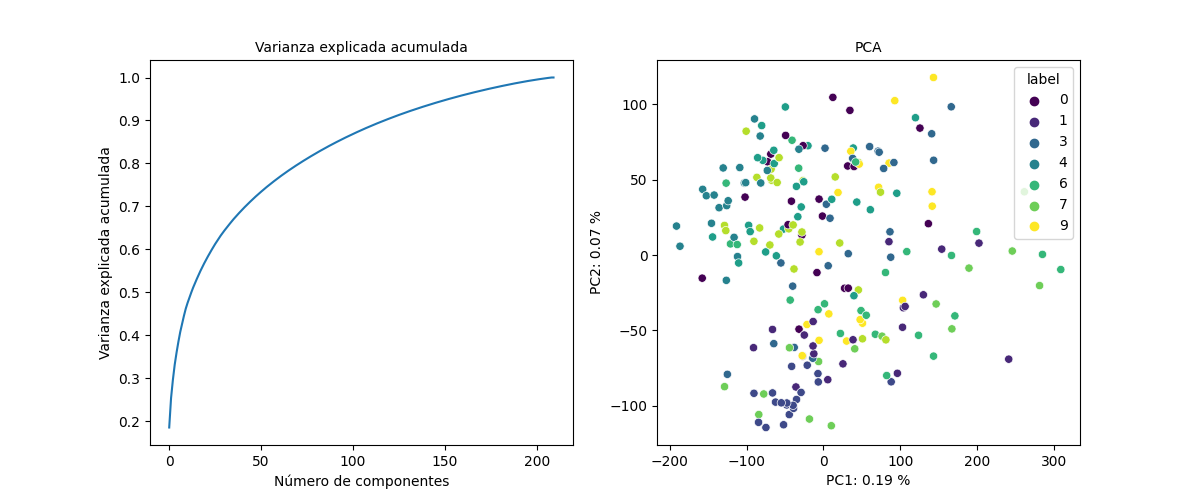
\includegraphics[width=1\textwidth]{9_1_pca.png}
  \caption{Análisis de componentes principales}
\end{figure}

%%%%%%%%%%%%%%%%%%%%%%%%%%%%%%%%%%%%%%%%%%%%%%%%%%%%%%%%%%%%


\end{document}